\documentclass[10pt,letter,oneside]{scrartcl} 
\usepackage{setspace}
\usepackage[utf8]{inputenc} 
\usepackage[english]{babel}
%\usepackage{raleway} \renewcommand*\familydefault{\sfdefault} %% Only if the
%base font of the document is to be sans serif
\usepackage{graphicx} % Required for including images 
\usepackage{enumitem} 
%Required for manipulating the whitespace between and within lists
\usepackage[T1]{fontenc} % Use 8-bit encoding that has 256 glyphs
%\usepackage{natbib}
\usepackage{breakurl} 
\usepackage[breaklinks]{hyperref} 
\usepackage{pdfpages}
\usepackage{endnotes} \let\footnote=\endnote

\usepackage[style=authoryear]{biblatex} 
\addbibresource{hack_entry.bib}

\usepackage{authblk} 
\author[1]{Luis Felipe Rosado Murillo}
\author[2]{Christopher Kelty} 
\affil[1]{Berkman Center for Internet and Society, Harvard University} 
\affil[2]{Institute for Society and Genetics,
          Department of Anthropology, and Department of Information Studies, UCLA}
\renewcommand\Affilfont{\itshape\small}

\title{Hackers and Hacking}

\date{}

\begin{document} \maketitle 

\section{Abstract} 

\doublespacing 

% From Gertaud:

% a) Starting point and relevance of the concept for cultural analysis,
% specific contribution in respect to digitization phenomenon.  b) Detailed
% presentation of the concept, discussion of key texts and (brief) history c)
% Example of a study which demonstrates in an exemplary way the analytical
% potential and practice d) Reception, critique and scope of the concept,
% potential further developments or trends e) Reference to other resources
% contributing to the understanding of these concepts such as blogs, wikis etc.
% (organized as a box at the end of the contribution)


\section{Introduction}

Hackers, either self-proclaimed or identified as such by peers,  are everywhere
to be found.  Twenty five years ago, ``hacking'' was one of a range of
underground practices, associated with a particular politics and defining a set
of individuals usually characterized as adolescent, white males obsessed with
computers.  Today, literally anyone could call themselves a hacker, or any
action a ``hack.'' In recent decades, we have experienced the extension of the
term to encompass many ordinary technical practices in various domains, such as
education, health care, humanitarian response, farming, parenting, bodily
modification, among many others.  Consider the current usage of the term
``hacking'' in the context of Internet companies in Silicon Valley, like
Facebook and Google, who elaborate a ``hacker way'' to call what they do
``hacking'' instead of (or in addition to) coding, engineering, and
entrepreneurship.  In public relation campaigns, hackers are described merely
as ``doers'' since ``hacking just means building something quickly or testing
the boundaries of what can be done'' (Funders and Founders.com 2013).
According to this very generous definition, we can all be called ``hackers'',
since we have been making artifacts for, at least, 2 millions years with the
creation of mode-1 stone tools (Clark 1961).

We have also witnessed a real proliferation and globalization of hackfests,
hackathons, and gatherings around the symbol of hacking for a myriad of
purposes, including but not limited to the design of Open hardware devices in
medical setting, the corporate-sponsored challenge of reinventing the soda
fountain with support from big companies such as Coca-Cola, the collective work
around public datasets to fight corruption or help with questions of public
administration, or simply coming up with an inventive use of a product that is
about to be released in the market.  Historically, hacker gatherings have
served the purposes of exchanging knowledge and bring small and fringe groups
of computer afficionados together, given the difficulty of finding peers to
share questions and findings when playing and working with information and
communication systems.  In the contemporary, many ``hacker marathons'' have
been organized by companies to identify programers for hire, offering
comparatively small sums as prizes for new software or hardware solutions which
would necessarily cost considerably much more on research and development.  A
new business has been created around the work of head-hunting for software
engineering talent under the rubric of the ``hackathon'', despite its original
connotation of a community-led sprint for developing technologies.

These facts suggest that the figure of hacking and hackers has become
fundamental to a contemporary technopolitical imaginary; but, at the same time,
it raises a question about what the anthropological study of computing should
look to in the future.  In this article we explore some of the challenges
facing the anthropological study of hackers and hacking.  We suggest first of
all that they are not necessarily the same thing:  the subjectivity involved in
cultivating ``hacking skills'' is not implicated in the range of things that
can be called ``hacks''---or put differenty not all hacks are perpetrated by
hackers.  This strange configuration of personhood, expertise, and practice is,
we suggest, familiar to  anthropology of technology generally, and also gives
us a window onto contemporary mutations of power and knowledge today.

\section*{Stories of Hackers and Hacking}

From the early 1950's experimentation with communication and computing systems
to the present-day hacker activist initiatives in the Global North and South,
the narratives on hacking has been reconstituted by different genealogies,
supporting different positionings with respect to whom and what counts as a
legitimate expression of hacking.  Most of these influential narratives have
been provided by journalists or hackers themselves, and not by scholars.
Canonical scholarly works are generally about the ``culture'' of
computing---and not specifically about hacking---which include those of Sherry
Turkle (1984; 1995), Diana Forsythe (2001); David Hakken and Barbara Andrews
(1993); Lucy Suchman (1987); Star and Ruhleder (?); Stephen Helmreich (1998);
Joseph Dumit (2004), and Greg Downey (1998). This literature has helped to
address the so-called ``myth of autonomous technology'' which pressuposes a
modernist ontology which separates it from human culture and society.
Pfaffenberger (1994) advanced the anthropological study of sociotechnical
systems with a refusal of assuming the separation between technology and
culture. In his studies of digital technology (the Usenet and the Personal
Computer as examples), he argued for the processual nature of technological
design as invariably embedded in cultural systems. With the exception
Pfaffenberger's and Turkle, little of this work is directly focused on hackers
or hacking as such, but nonetheless constitutes some of the most significant
ethnographic studies of computing in English-language.

The journalist Steven Levy is one of the most authoritive sources of the early
history, published in his mid-1980's book \emph{Hackers: Heroes of the Computer
Revolution}.  Levy's work is examplary in offering early heroic narratives of
exploration of computer systems based on life-histories, tracing the origins of
the hackerdom to the students' group ``Tech Model Railroad Club'' (TMRC) of the
Massachusetts Institute of Technology (MIT) of the 1950's. \emph{Hackers} has
been translated in several languages and accepted among distinct hacker
communities worldwide. Its narrative had the performative force of instituting
a return to the figure of the ``virtuous hacker'' in the contemporary with its
descriptions of the experience of early hackers around research centers at MIT
and Stanford, Northern California collectives such as ``People's Computer
Company'' and ``Homebrew Computer Club'', and companies such as Apple Computer
and Sierra Games. Levy has also popularized a positive definition of hacking as
grounded in the ``hands-on imperative'', the need for information freedom (as
to facilitate technical exchange and promote further hacking), the rebelious
attitude with respect to authority, centralization, and control of computing
infrastructures, and the idea that technical work could be used to bring forth
beauty and effect positive social change (Levy 1984).

A more recent account of the early origins of hacking was given by the
technologist Phil Lapsley (2013) in his book \emph{Exploding the Phone: The
Untold Story of the Teenagers and Outlaws who Hacked Ma Bell} which
reconstructed the early history of ``phone-phreaking'', the precursor of
computer hacking which consisted in the exploration and information sharing
about phone systems.  Lapsley describes a genealogy which connects the direct
action of Yippies of the 1960's autonomist movement with exploration of
information and communication systems in the context of corporate control and
centralization of computing in the 1960's and 1970's.  His account calls
attention to a fundamental aspect of phone phreaking: a shared experience in
which the telephone became the very embodiment of curiosity, and the phone
network, a space for exploration, discovery, and socialization.  This is an
important period of transition of the past 50 years in which we have witnessed
the passage from large-scale, military-grade computer infrastructures to
distributed personal computing power with massive network integration in the
Euro-American world. The consequences of this transition are key for the study
of digitization: the transformation of cultural practices through the usage of
digital technologies, difference in infrastructure (of computing networks),
materiality (of computing devices), and virtuality (of archival and social
memories).

Hafner and Lyon, Where Wizards Stay up late. 

Raymond and auto-ethnography

A distinctive feature of hacker collectives resides in their effort of
self-organization around publications and gatherings.  Akin to other
independent groups, many phone-phreaking and hacker groups engaged in the
practice of self-documentation, with the publication of ``electronic zines'',
manifestos, and, in a few cases, with the enthusiastic adoption of an
anthropological and historiographic mode of inquiry.  The work of Eric Raymond
is regarded as one of the native anthropologies of the hackerdom with
publications on the community around the UNIX operating system (2004), the
``Jargon File'' which documents the local dialect of MIT hackers in the
\emph{New Hackers Dictionary} (1993), and the collection of influential essays
on the benefits of Free Software distributed and collaborative software
development model for corporate audiences in \emph{The Catedral and the Bazaar}
(1999).  Yet another native scholar who has done an extensive archival work of
computing cultures is Jason Scott (see Appendix), who has done considerable
work in maintaining online archives of electronic documents, series of
life-histories on hacking, Bulletin Board Systems (BBS), and adventure,
text-based games.

Two major sociological and historiographic contributions in the literature
depicting the rise and fall of the "hacker underground'' of the 1980's and
1990's were ``Hacker Culture'' by the communications scholar Douglas Thomas
(2006) and ``Hackers'' by the sociologist Paul Taylor (1996). These two books
are complementary in the sense that they describe the underground hacker scene
of the United States and the United Kingdom in the period of popularization of
hacker techniques and criminalization of its practice. Taylor's work is focused
on the relationship between the nascent computer security industry of the
1990's with the computer underground, which is a fruitful description of the
duality which is characteristic of the underground lifeworld in which hackers
are both the chaser and the chase, both on the side of law enforcement and on
the side of the curious hacker collectives, navigating the thin line, most of
the time indistinguishable, between the harmful and the inocuous, the virtuous
and the vicious with respect to the impacts of the exploratory attitude of
computer experts.  Douglas' work is particularly useful in describing the
discursive strategies in which the figure of the hacker as a unpredictable and
uncontrollable ``criminal'' was instituted -- having created a mythology around
the alleged superpowers of curious adolescents with access to a personal
computer, a modem, a phone line and certain access to information about flaws
and holes in computer and communication security.

The work of the science-fiction writer Bruce Sterling alongside others in
creating the ``cyberpunk'' literary genre led him to cross paths with hacker
groups in the United States in a key moment of its history: the late 80's and
early 90's in which the wave of ``crackdown'' on hacker collectives has become
widespread. His book ``Hacker Crackdown'' narrates the story of police chase
after teenage hackers.  Key in his depiction is the argument of how misguided
the police attempts were in framing computer hacking as a serious criminal
offense without understanding of the practice and its consequences. 

There are several names that raise to the ranks of media darlings and misfits
in this context as well.  One of the biggest names is that of Kevin Mitnick,
who became the mainstream media martyr after an incredible story of playing
cat-and-mouse with the federal police in the United States.  After been
arrested, a mobilization of hackers around the slogan ``Free Kevin'' took over
the computer underground to clarify the misguidance and overreach of
prosecutors in Mitnick's case.  His name became well known given the
specularization of his case in the mainstream media with the guise of the
``Most Wanted Hacker''.  Many other hackers' stories rose to prominence in this
period, including the hacker collective Legion of Doom (LOD) and their New
York-based rival off-shoot Masters of Deception (MOD).

After Levy's book Hackers with the key elements of the moral order of pioneer
hackers, discussions of the "hacker ethic" were popularized in the late 1990's
with the publication of the "Hacker Ethic and the Spirit of Information Age" of
the Finnish philosopher Pekka Himanem (2001). The book is important for calling
attention to the subjective dimensions of a cultivation that is distinctive of
the computer hacker ascesis.  It falls short, however, in its lack of empirical
grounding.  In response to the generalizations of the "hacker ethic" in
Himanen's work, Golub and Coleman (2009) argued for the treatment of "genres"
of hacking as to get at distinctions with respect to the moral and technical
orders different hacker groups inhabit. 


Benjamin Nugent on Nerds % read it, but it feels a bit anecdotal to me

Work in 2000s by Coleman, Golub, Kelty, Nardi, Boellstorff, Johns, Juris...  %
I am afraid
									     % we
									     % might
Coleman and Golub, Genres, as an essential distinction.                      %
go over the
									     % page
									     % limit

Coleman Ethnographies of the Digital

Shifts towards questions of amateurism/expertise, participation and personhood. 

Another important piece of hacking history has been investigated by
anthropologists under the guise of the Free and Open Source technologies of the
past thirty years. Two major contributions on this are ``Two Bits'' by Chris
Kelty and ``Coding Freedom'' by Gabriella Coleman. The former provides the
basis for the analysis of the historical formation of a new kind of publics
which has a distinctive charateristic of recursivity, that is, it is defined by
a group of active computer technologists whose means of organization relies on
the need of openness and possibility of redefining and reorganizing the very
means of association. This work has been central for the study of a new phase
of hacking under the rubric of Free Software as an emergent moral and technical
order, as well as a new mode of production of information technologies. Equally
important for the literature on hacking, Coleman's work emphasized the moral
and legal cultivation through which software developers of a particular Free
Software project, Debian GNU/Linux, are exposed in participating in the
collective effort of building an entire operating system by self-organizing a
large remote enterprise over the Internet. Both authors pioneered the
investigation of the liberal underpinnings of Free Software as a
technopolitical project as well.

More recent publication and public debates around Free Software and hacker
communities has shifted the focus to questions of gender discrimination and
imbalance.  Alongside the work of feminist and women hackers around computer
collectives such as Systers, LinuxChix, Ada Initiative and Geek Feminism, new
publications have addressed the  question of extreme disparity in Free and Open
Source projects where it is estimated that less than 2\% of the contribors are
women and other gender minories (Ghosh et al.  2005).  Nafus (2011) has
discussed the question of gender with respect to the ways in which the
organizing symbol of ``openness'' represents more than an alternative to the
intellectual property regime and a mode of managing the collaborative efforts
in software development. According to the author, the question of openness is
accompanied with the insistence that gender plays no role in software
development, serving in fact to disguise the mechanisms of exclusion of women
and gender minorities from Free and Open Source projects.  These mechanisms
include but are not limited, to the maintenance of design decisions which
demand previous technical knowledge, excluding newcomers; the creation of new
expressions of masculinity that are exercised through public argumentation and
defense of one's technical prowess, which are alienating to women and other
gender minorities; and, last but not least, one of practical effects of
``openness'' which consists in denegating or outright denying ``difference''
for the sake of unfettered circulation of code, which has the effect of
generating ``flame-fests'' when the question of gender is posed for debate
among FOSS developers. 

Nicolas Auray    % only read him with respect to debian, one article...

Sebastian Broca   % haven't read him... but I want to.

The most recent publication on the topic of ``hacking'' has been published in
France by Michel Lallemand on the topic of ``hackerspaces'' and the rise of the
discourse and practice of ``making".  Lallemant has offered an ethnography of
the "maker movement'' in the San Francisco Bay Area with a focus on the
question of the transformations labor and its reorganization with the creation
of independent spaces for collaborative work with digital technologies. The
book describes the community space ``Noisebridge'' in San Francisco which has
been one of the most influential autonomous spaces for the recreation of
hacking as a political symbol for self-organization and democratization of the
access to expert computing knowledge around the globe.


\subsection{Hackers...}

Are hackers representative of a distinctive elaboration of the modern and
liberal notion of the person?  This question is open for further inquiry across
different political and philosophical traditions outside the Euro-American
world, aas most of the literature is focused on North American and Western
European hacker collectives.  Other than the central questions of autonomy and
privacy, the modernist notion of self-development is a common thread linking
different hacker collectives.

There is a tendency to think of hackers first as a subculture with specific
forms of affiliation and a sense of belonging to a community.  But central to
this identification is the existence of the ``hack'' and the so-called ``hack
value'' (Raymond 1993) which specifies the former.  Hackers are said to have a
culture of perpetrating a particular kind of act which can supposedly be
distinguished from the actions of other kinds of people in other communities
(especially, those in bureaucracies, hierarchies, corporations, or other
hidebound organizations of the past).  The ``hack'' however, can be mobile and
re-usable, it often, but not always, takes the form of a tool or set of tools;
it can be a one-off, round-about way of getting something done, but it is often
something that is re-usable, which serves as yet another element for
generalization.  Many ordinary practices of repurposing, which in different
contexts have different expressions, such as the ``gambiarra'', the Brazilian
term for an improvisation or ``hack'', the ``juugad'', which expresses a
similar improvisation of technical nature in India, and the ``shanzhai'', which
is a more specific form of repurposing in mainland China of mobile devices.  In
these cases, the ``hacker'' persona is troubled by the recognition that
``hacks'' are frequently borrowed, re-used, reconfigured and redeployed by
people who only subsequently come to think of themselves as hackers---or maybe
don’t do so at all.  If you pull off a great hack, depending on the context of
occurence and the participants of the exchange, you could be called a hacker
regardless of your expertise.

Such a complicated identification of who counts as a hacker poses a dual
problem for anthropological research.  On the one hand, it creates a challenge
for making sense of personhood itself in an era where conventional idioms of
identity are being contested in this way; on the other it deflects our
attention to this act itself---``hacking''---and to the question of what it is
and how it might be studied anthropologically.  Are the actions of pirates,
activists, criminals, cyber-activists, and other such figures ``hacks''?  Why
do people call mid-level engineers, librarians, scholars and designers
``hackers''?  Do all of these people share a particular disposition of
personhood, or do they share a milieu of technologies, material and
institutional forms at their disposal?  How can we disentangle the sudden
dispersal of hacking and hackers, in the sense of a wide circulation of
devices, persons, and discourses, around the world?

As we briefly exposed in the previous section, there have been competing
definitions of hackers.  Consider two distinctive definitions: one from the
Internet engineering community and the other from ``hacker underground.''  For
the former, a hacker is defined as a person ``who delights in having an
intimate understanding of a technological system,'' whereas his or her
opposite, a ``cracker,'' is an individual who attempts to access computer
systems without authorization.  These hackers pride themselves on building
complex systems out of available parts, or on getting around an engineering
problem in a simple and elegant way.  As Coleman (2012) details, they are both
highly individualistic in the Euro-American context, but oriented towards a
community of other hackers.

By contrast, for underground hacker collectives, hacking may signify
exclusively ``systems' penetration'' and exploitation as a display of technical
ability and mastery or, increasingly, for monetary gain.  For them, hackers are
people ``who gain unauthorized access to computer systems,'' a practice which
is evaluated in terms of technical aptitude and virtue, measured up against the
value of contributions in software code, information, and documentation.
``Exploits'' become objects of value that circulate--at one time only for a
kind of cultural capital amongst hackers, but increasingly today as part of a
robust market for ``Zero-day'' exploits (Soghoian xxxx).  Increasingly, these
forms of hacking are also well established in the military and defense world,
both defensively and offensively.

Members of the early Internet engineering expert communities claiming the
hacker status would strongly disagree with the definition given by or of the
hacker underground. Many of these communities were described in the origin
stories of Free and Open Source development as a ``natural attitude'' of
pioneer computer technologists.  They are strongly associated with research
universities and with a certain mythical understanding of scientific method and
practice; they point back to avatars such as the Digital Equipment Computer
Users' Society (DECUS) in the sixties, or SHARE, the IBM mainframe computer
users' group (Akera 2007), the MIT community around the Tech Model Railroad
Club, the Artificial Intelligence Laboratory operating system development
staff, and the early community around Berkeley Unix System distribution, among
many others.  The period which extends from the 1950's to the 1970's is
identified in the literature with the work of early, pioneer hackers in pushing
the boundaries of computing on many fronts: from hardware hacking to personal
computers, from new operating systems to video-games and graphical user
interfaces as we discussed above.

By contrast the ``hacker underground'' has its own mythical histories,
associated with the history of phone phreaking, bulletin board systems (BBS),
zines like ``2600'' and ``Phrack'', and movies like \emph{War Games} and
\emph{Hackers}.  These stories are more likely to reference the criminalization
of hacking under the US Computer Fraud and Abuse Act, and the fabled exploits
of people like Phiber Optik, Kevin Mitnick, Dark Dante, Erik Bloodaxe, and many
others.  While many Internet Engineers will point to Stephen Levy's
\emph{Hackers} as canonical, the hacker underground may point to Bruce
Sterling's \emph{Hacker Crackdown}.  Over the years, these two versions of
hacking have competed and collaborated: they cross paths at conferences like
DefCon, Chaos Computer Congress, and Hackers on Planet Earth, as well as at
major Free Software and Open Source events worldwide.  The \emph{cause célèbre}
of intellectual property activism amongst hackers--Dmitri Sklyarov---was
arrested at DefCon 9, but became a symbol for hacking as political
form---''code is speech'' (Coleman 2009). 

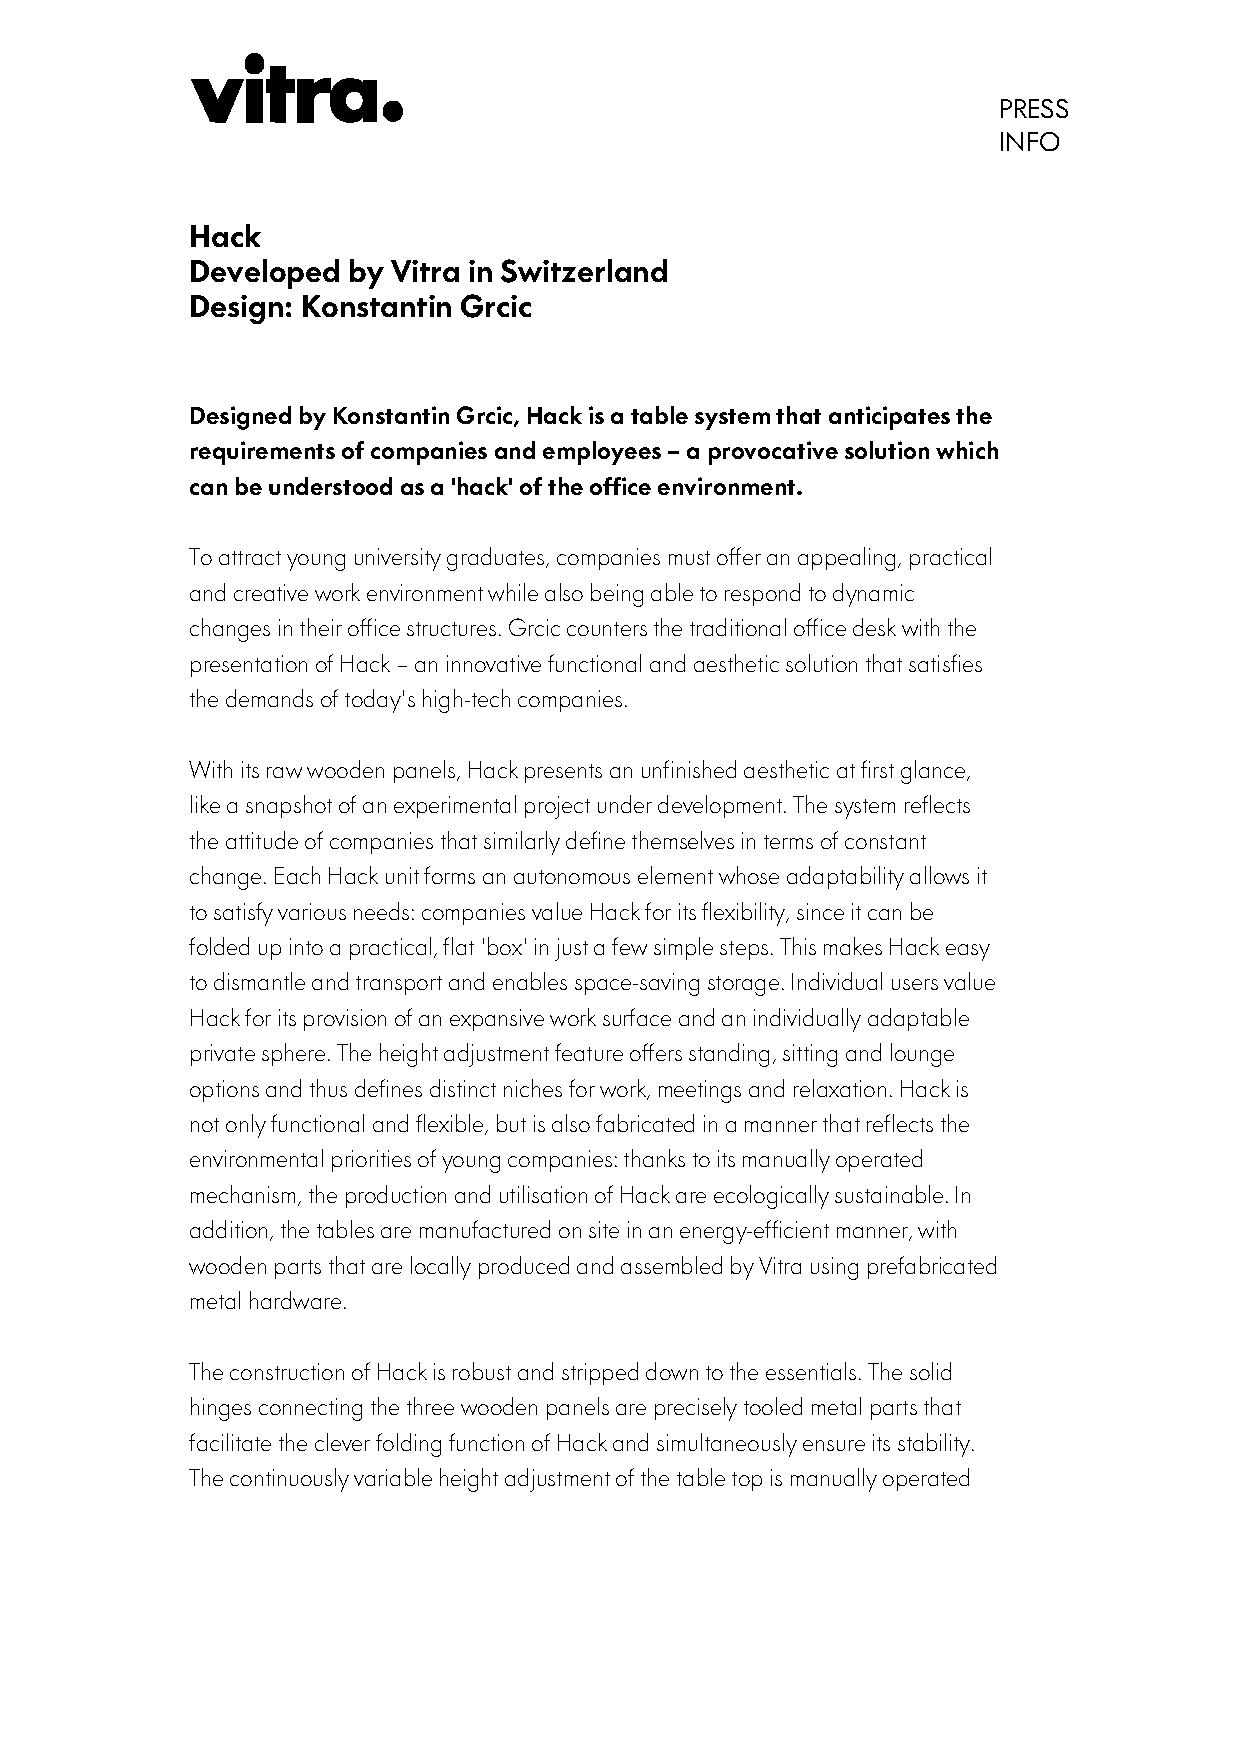
\includepdf[pages={1,2},nup=1x2,scale=0.75]{images/Vitra_Hack}

\begin{figure} \centering

\includegraphics[scale=0.6]{images/Workspirit13HACKStudioAKFB3}

\includegraphics[scale=0.4]{images/HackDeskGrcic} \caption{The Hack Desk,
designed by Konstantin Grcic, manufactured by Vitra.} \label{fig:hackdeskimage}
\end{figure}

Both of these communities reject with derision the widespread use of the term
today in mainstream culture.  Facebook employees who ``hack'', ``brogrammers''
in Silicon Valley, and the generalized use of the term ``hack'' to mean ``do
something'' are seen as corruptions of various competing versions of a
tradition.   The Vitra ``Hack'' desk (See Fig), for instance, performs an
attentuated and distorted version of hacking that emphasizes Silicon Valley
neoliberal start-up culture, an ``individually adaptable private sphere,'' and
a vision of flexibility in which the desks convert into sofas as part of a
longed for collapse of work, leisure and political authenticity, primarily
amongst white, upper middle class technology employees in Europe and North
America. 

But the mainstreaming of hackerdom is just as likely to expose the sexism
and/or racism of past communities of hackers.  An ``elite hacker'' in an
interview to an influential hacker zine declared the demise of the hacker
underground with the xenophobic and mysoginistic observation that ``"today it
is claimed that the Chinese and even WOMEN are hackers. Man, am I ever glad I
got a chance to experience "the scene" before it degenerated completely"''
(Phrack 2008).  Symbolically violent in its own terms, this observation indexes
not only the ethnocentric and gendered lifeworld of most hacker collectives,
but the fact that hacking is no longer limited to the virtual play-fight among
Anglo-American suburban adolescents, pointing also to questions of personhood
with the evaluation of who gets to be considered a hacker.

What is important to emphasize in these examples is not the adoption of one
definition or another, but the evidence of a series of disparate, conflicting,
and generative differences for the contextualization the hacking. This is the
evidence of an oscillation in respect to the value of ``hacking'' over time:
fluctuating from positive to negative moral valences, that is, from elite,
exclusive groups of technologists to online and offline communities marked by
the rhetoric of opennness and transparency, or, from what the communications'
scholar Douglas Thomas called the ``culture of secrecy'' of the hacker
underground in the height of the cold war to a ``culture of collaboration,
openness, and transparency'' as a shared utopian horizon in neoliberal times.

\subsection{...or hacking?}

Is ``hacking'' a distinctive kind of action?  What differentiates it or gives
it consistency today, and how might it be related to leaks, breaches, or other
actions of information disclosure, circulation, both constructive and
destructive?

Leaking, for instance, has become associated with hacking in the last decade.
The furor around Wikileaks, for example, brought the fun-loving underground
anti-collective Anonymous to world-wide attention via its coordinated attacks
on corporations and governments.  Similarly, sharing or piracy: The May 15
movement in Spain was spearheaded alongside protests of La Ley Sinde---an
anti-piracy law widely opposed by musicians and consumers alike, and ultimately
merged with anti-austerity protests of the ``Indignados''; key activists in the
North African revolutions were also involved in the movements organized by
Anonymous and were often connected to actors in both May15 and Occupy, as well
as hacker activists of many groups including the group ``Telecomix''.  Occupy
movements around the globe borrowed tactics, technologies, slogans and ideas
that both explicitly and implicitly reference Free Software, the Pirate Party
and copyright reform movements—--all of this at the same time that US and
Israeli spies were infecting Iranian nuclear power plants with the StuxNet
virus (Zetter 2014), and the NSA and GHCQ were cataloguing all of this, and
perpetrating some of the greatest ``hacks'' the internet has ever seen---and
this we know mostly because of the even greater intelligence leak of Edward
Snowden.

Hacking, as a practice, is not confined to hackers, but increasingly a practice
essential to the social fabric in surprising ways.  One might turn to
``practice theory'' in its various forms to explore this---are hackers a
``community of practice?'' Or constitute an emergent political expression of a
particular sociocultural formation? Are they heterodox actors in the context of
the computing field or are they wildcards in various professional domains, akin
to the figure of Luther Blisset or Guy Fawks who can come in and out of a
mysterious identity?  These questions would combine questions of technical and
political cultivation with the identification of a distinctive practice in
order to suggest that the identity of a hackers is based in the practice of
hacking.  Indeed, such definitions are common (we ourselves have proposed
them---in the case of a ``recursive public'' for instance Kelty 2008).  But
this approach cannot accomodate the fact that hacking and hacks have become
more obsteperous and unruly in their circulation: hackers fight hackers and
trolls troll trolls and pirates steal from pirates today.  To conflate the
question of identity with the question of the practice, political, technical or
otherwise, would miss the mark.

Instead, there are a diversity of moral and technical orders inhabited by
people who are called or call themselves hackers. From the underground hacker
collectives to ``grey hat'' security researchers to spam-slinging criminal
hackers, to the hard-core free speech and privacy cryptography defenders; from
the die-hard Free Software activist to the business-oriented Open Source
evangelist; from the über-cool Northern European art hackers to the
goofy-but-terrifying Anonymous hackers, and so on.  As Coleman and Golub (2009)
point out, there is no single liberal ideology that hackers adopt, but rather a
range of ‘genres’ in which any given individual or group might operate,
implying both the freedom and the constraints that word signals.

But what is the substance of these moral genres?  We argue here that these
``genres'' are not about identity or collective belonging or community.  They
are about specifiable practices to be sure, but they are bound up with new
kinds of technological affordances that make practices less dependent on
embodied skill than many other kinds of practice (e.g. glass blowing or cabinet
making) and as a result more mobile and modifiable.  The expanded field of
hacks, leaks, exploits, breaches, ops, online campaigns and so on form the very
substance of political life today in its complex entanglements with things,
protocols, perspectives, and sensibilities of digital technologists and
technologies.

--> explain here that the anthropological reason to do this is to refine our
ability to track and observe practices of power in ways that go beyond the
simple Foucauldian model of sovereignth, biopower and exception.  To add to the
repertoire of tools anthropologists themselves use in order to analyze power
amongst different social actors.  

{  And especially: that it is about how techniques are recombined in a topology
of power, not just the epochal shift of regimes of power.   It is this active
``recombination of elements'' that Foucault recognized as a way to stretch,
transform or warp the patterns of correlation that make up a given topology of
power. What better indication of this deformation of topology than the fact
that today the pirates see themselves as having a coherent political platform
while the social movement activists of Occupy claim not to.}

``Hacker practices'' don’t always originate with hackers, nor do they confine
themselves to use by hackers.  Tactics or practices are picked up by computer
security scientists and researchers, security firms, police forces, political
campaigns, anti-piracy outfits, analysts of all sorts, as well as spreading
globally through networks of activists, hacker and maker spaces, legal firms,
musicians and artists, or consumers and pirates. Hackers go to work for Google
or Facebook, anti-piracy companies appropriate the tools of hackers and
pirates.  Power, in this sense, is about the recognition, appropriation,
recomposition, and redistribution of tactics and practices: not ideologies or
genres--but recomposable instances of power.  The technique of DDOS attack, for
instance, or the use of a cease-and-desist letter, the creation of
commons-producing copyleft licenses, or the use of the BitTorrent protocol can
all be identified with hacking, but they are not all of the same kind.
Building on the work of Coleman and Golub (2009), we offer a brief proposal for
a set of distinctions that might make sense of these differences, and
generalize the generic categories they offer in order to expand the analytic
possibilities.  The first three practices listed here (invention, inversion,
and figuration) are quasi-direct forms of action; they are accessible to
anyone, even if the barriers are significant, and do not require significant
investments of money or organization to achieve.  The last two (regulatory
action and force), however, are often more second-order or ``representative''
in that they often require physical, financial or organizational resources and
a certain scale and depth of involvement to perform. 

% I am not sure what to do with this "accessible to anyone"...  when the
% distinction here is "signficant investments of money or organization"


\subsubsection{Invention}

Invention includes building and making things, and not only material things,
but so-called ``immaterial'' products such as software or organizations.
Invention is intended to cover those practices that arise out of a lack or out
a sense of need of some sort; where there is no clear need, there is
nonetheless a recognition of possibility based in the existence of multiple
existing tools and components.  So, creating software, hacking together
hardware components or starting up an organization are all practices of
invention in so far as they are carried out to solve a problem or respond to a
lack that makes certain possibilities clear.

Invention as we use it here implies a material culture of ready-made,
accessible, often lego-like parts---and not the fabled \emph{de novo} creation
of a technology or idea.  It implies easy access to tools (recall the ethic of
the Whole Earth Catalog: ``Access to Tools'' described by Turner 2006), mutual
aid and instruction and an appreciation for both the DIY possibilities of our
world, and sometimes a respect for (and desire to contribute to) the
coordinated engineering necessary to bring them into being.

Furthermore, the practice of invention implies an affinity based in shared
understandings of how things work.  Whether that is a classic engineering
culture (based in University and/or corporate practice), a DIY geek culture, a
UNIX culture, a glass-blowing culture (O’Connor ????) or whatever, invention
demands not only skill but the capacity to recognized others with more or less
the same skills, habits of practice and commitments to certain kinds of
technological or material choices (Sennet 2008).

\subsubsection{Inversion}

Inversion is a term meant to signal a practice that---at least under the label
of ``hacking''---is often insufficiently distinguished from invention.
Inversion is the kind of hacking that involves finding and exploiting
vulnerabilities, using systems against themselves, inverting the intended
purpose of a system, or remixing one for purposes of critique, parody, ridicule
or something more practical (Galloway and Thacker ???).  In terms of hardware
it includes the practices of modding and customization; in terms of software it
includes the practice of finding and exploiting weaknesses in software (for
good or evil intent) or recombining software elements in a surprising and
clever way in order to achieve a new goal.  In legal terms the most famous
``inversion'' is the General Public License (GPL), which uses existing
statutory copyright law to accomplish something it was not intended to do.
Wikileaks is in some ways a practice of inversion, insofar as it makes public
information not intended to be. 

Inversion implies institutional structures or infrastructures with a certain
transparency (one must be able to see how something works in order to exploit
it).  Where that transparency is absent, at least some route towards
reintroducing it (leaking documents, reverse engineering, etc). The debates
about secrecy and transparency are very often deeply engaged in a particular
form of inversion---but as we will see, also engage in the tactic of
figuration.  Inversion also implies faith in engineering and in the rule of
law: for something to be inverted is not the same as for it to be destroyed.
GPL licenses work because copyright law is legitimate and enforced.  Remix or
recombination of software is done because the challenge is to make something
work better or meet higher standards of practice.  By extension, the faith is
that things can always be and become better—only imperfect things can be
hacked, inverted, in this sense.

Similarly inversion implies patterns of regularity that can be exploited---the
very thing upon which the practice of invention often depends as well.
Inversion works upon certain technological or organizational preferences shared
amongst a large group of people---for instance the use of SCADA control systems
amongst process engineers who design large industrial plants allows for hackers
to imagine exploits with powerful effects on the material world.  Similarly,
entrenched social behaviors are often exploited in ``social engineering'' hacks
that rely on the regularities of organizational design and human behavior.

\subsubsection{Figuration}

Figuration is a term meant to capture the more traditional and recognizable
forms of political action: rhetorical persuasion, ideological argument,
political advocacy, etc.  Classic descriptions of the functions of the public
sphere tend to characterize it as an issue of sovereignty---the ability of
``the people'' to speak to and force changes amongst established domains of
power like the state, the church, the military, etc. (B. Anderson ???).  All of
the tactics involved here are about visibility and the legitimacy of a
political process.  In eras or locations where there is nothing like a
legitimate democratic government, tactics of figuration are often ineffective
or irrelevant.

Materially speaking, figuration also depends on shared communication
structures---and this is where the overlap with the tactics of invention or
inversion are most intriguing.  When communication practices are invented or
inverted in response to weak practices of figuration.  Longstanding
institutional structures (such as public hearings or requests for comments)
both facilitate and provide friction on the practice of figuration.  Figuration
also implies a stable set of narratives---what Charles Taylor dubbed social
imaginaries---against which it is possible to make arguments, whether rational
or emotional, which have political efficacy.

Traditional institutional structures of government, such as new political
parties, as well as emergent ones are focused on figuration. Non-governmental
organizations engaged in policy analysis or advocacy, social movements engaged
in protest, or scholars engaged in criticism and research all work at the level
of figuration, in part because it has traditionally worked at the largest
scale—that of the public sphere or civil society.

Substantively (at least in the domains of intellectual property and information
technology) practices of figuration have been heavily focused on issues such as
privacy, transparency, free speech, freedom to operate (or innovate) and
network neutrality.   These issues subtend a long and rich discourse that
includes both scholarly debates and conventional understandings of these
concepts and their value to our lives. Examples of figuration include the
Electronic Frontier Foundation, which was created in the context of ``hacker
crackdowns'' of the early 1990's to articulate a discourse on the importance of
defending civil liberties online, primarily organized as a fund to legally
defend hackers from prosecutorial overreach. Other examples include the
Creative Commons intiative which created an alternative to the copyright law by
creating a set of flexible copyright licenses to bypass intellectual property
restrictions, while fostering a digital commons; and the Tor project as an
experiment in computer network routing that became an important project and
site for defense of anonymity and privacy online, especially in the context of
mass survaillance programs and ostensive monitoring of Internet communications.

\subsubsection{Regulatory action}

Regulatory action includes any form of policy change intended to introduce,
maintain or extend control.  State-based forms of regulatory action are the
most obvious and familiar but large corporations also engage in regulatory
action of particular kinds routinely---especially those industries who control
networks or technologies in widespread use.

Regulatory action implies large bureaucratic organizations of a classic
Weberian type---rule-based, hierarchically ordered, and subject to regimes of
oversight and transparency.  As a result, regulatory action is relatively rare,
and comparatively complicated to carry through.  The tactics of invention,
inversion and figuration are often oriented towards influencing, responding to
or disrupting regulatory action of various kinds---the 2012 case of protests
against SOPA/PIPA being a clear case; another case would be Operation Payback
conducted by members of Anonymous against the global credit card companies
Mastercard and Visa, who had engaged in the regulatory action of systematically
blocking PayPal donations to the Wikileaks organization. 

Regulatory action also implies a professional cadre acquainted with the rules
and procedures of these organizations, oriented towards professional norms of
democratic governmental practice, even if in practice such norms are honored in
the breach or routinely subjected to the power of external interests.
Nonetheless, regulatory action is something that is routinely pursued
strategically by different groups---a corporation lobbies congress, one groups
sues another or asks a court for an injunction; lawyers send letters; states
create new roles and appoint people to them (e.g. IP Czar); courts mete??? out
punishment, etc.

Inversion often borders on regulatory action when it is used strategically to
achieve something in the interests of a particular entity, but so too does
figuration, which is often the tactic most often employed to support or protest
a proposed legal change (both were used in the case of SOPA/PIPA).  Cases of
significant interest include those where regulatory action look more like cases
of inversion---i.e. where a legal action, for instance, is used to threaten,
intimidate or censor a particular group. The injunctions filed against
MegaUpload and Kim Dotcom, for instance, are represented as mere enforcement of
the law, but in reality represent the effective organization of state power by
industry organizations like the MPAA and the RIAA.

\subsubsection{Enforcement(s)}

Finally, there are practices of enforcement. Often only implicitly or
metaphorically included in a Foucauldian analysis (discipline is held to be
more insidious and more profound kind of force, a 'government of the soul' for
instance).  While classic displays of sovereign power are relatively rare
(helicopter raids by anti-terrorist forces on New Zealand mansions of
flamboyant wannabe hackers notwithstanding in the case of Kim DotCom), they
remain a central tactic in the repertoire of power, and they are by no means
restricted to a state and its soldiers and police forces. 

Many forms of enforcement are widely available today.  A range of tactics and
practices of which the DDOS is only the most common are not confined to any
particular segment of society, but available to anyone who might, for instance,
download and install a copy of the Low Orbit Ion Cannon (or its predecessor,
organized by the Electronic Disturbance Theather group which in 1994 created an
application to flood the Mexican government website with requests to send a
message in support of Zapatistas).  Legal tools like cease-and-desist letters
are also routinely used as a tactic of force; even patent litigation can be
figured this way when conducted by so-called patent trolls.  Networked-based
forms of disruption are very often simultaneously tactics of invention or
inversion—coming into existence in response to the actions of states or
corporations.  Piracy and cracking generally might be said to move from being a
tactic of inversion when a vulnerability in a copy-protection scheme is merely
demonstrated (e.g. Sklyrov demonstrating holes in the eBook Reader) to a tactic
of force when that vulnerability is routinely exploited.


\begin{figure} \centering 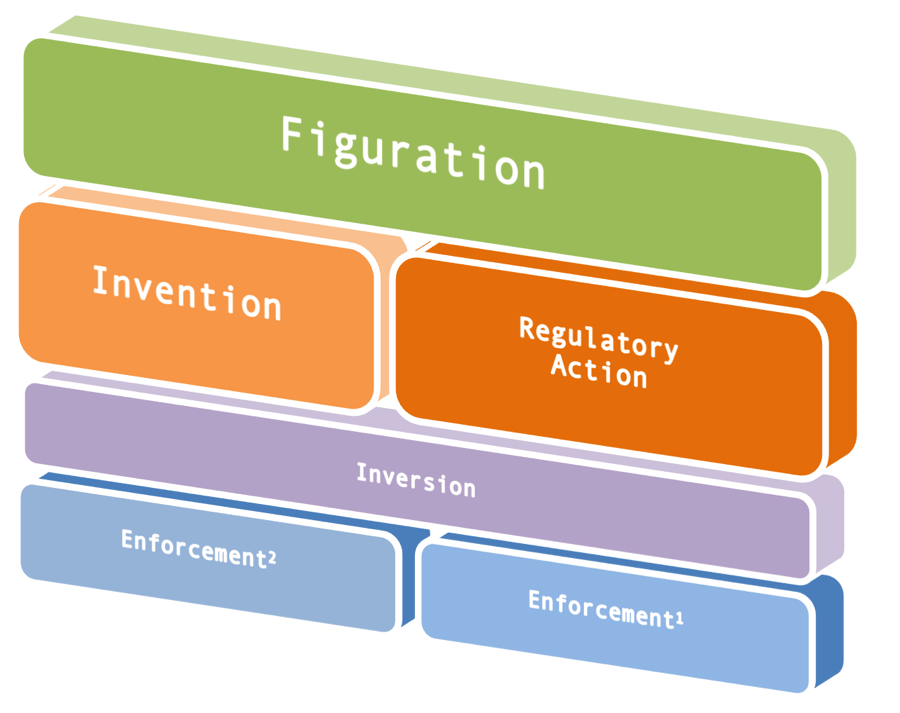
\includegraphics{images/protocolstackV2}
\caption{Protocol Stack of Power: an analytic decomposition of hacking
practices and how they might relate} \label{fig:ProtocolStack} \end{figure}


How do all these practices fit together?  As a ``topology'' perhaps, in which
different techniques emerge in response to others, and to events and
thresholds, both political and technological.  Inventions and inversions often
come in the face of regulatory actions and their enforcement -- the case of
Napster and BitTorrent in response to the DMCA for instance; or the figuration
of hacking in response to the Computer Fraud and Abuse Act of 1986; or the
inversion of the GPL in response to the enformcement of conventional IP law.

Figure x suggests that hacking today takes the form of stack of pratices
available to different actors at different times, but responding to specific
technological and political affordances.

%How does the moral and technical cultivation of hackers (of different
%persuasions) connect to this stack of practices?  In what ways can we
%understand the ethical %cultivation of particular kinds of skills (skills of
%invention, inversion etc.  vs. those of figuration or regulation) as leading
%to different forms ?  Does this topology remain stable?    

The question we end with concerns the dynamism of this topological stretching,
and the production of stability.  Just because the contemporary moment is one
of exacerbation and failure does not imply that we have entered the epoch of
uncertainty---rather the question is: constant oscillation or stabilizing
configuration.  History favors the stabilization of forms of power, but the
manifest speed and ease with which the contemporary topology can be stretched
and deformed suggests a perpetual oscillation or turbulence, limited only by
the energy and enthusiasm that can be committed to the various practices of
invention, inversion, enforcement or regulation.  


\section{Hacking and Digitization: Open Questions}

{\bf Imperial imperative of digital technology} to transform sociotechnical
difference through contact into its ressemblance (or poorly made copy).
Anthropological studies of the global circulation of digital technologies and
expert technologies have demonstrated the naturalization of Euro-American
underlying assumptions in digital design: from user interfaces to data models;
assumptions of usefulness of particular technologies based on the prestige of
their place of creation; and the imposition of particular projects from centers
of production to disconnected peripheries of the global South.

% --> I would add here: how is the global difference in personhood of hackers
% related to the global accessibility of hacks?  What are examples of the
% reverse process, where the actions of global hackers (say, book pirates in
% russia or activists in Tunisia, or Anonymous' attacks on ISIS) have an impact
% on mainstream practices?

{\bf Power imbalances, gender and ethnic troubles.} One of the key markers of
difference among computer experts concerns gender and the exercise of
particular forms of masculinity in heated arguments around technical issues. It
is key for displaying structured relations of power and practices of value and
worth assessment within hacker communities.  Questions of power and difference
refer to the nature of sociotechnical ties within expert communities. In this
sense, hacker collectives imagine themselves as meritocratic orders for having
instances in which merit is recognized and rewarded through vetted collective
mechanisms, but it is also oblivious to unequal starting points for the
development of tech skills for participation in hacker collectives, such as
Free and Open source projects. The gender question in digital communities is
open for empirical study since most of the literature on hacking has dedicated,
at most, footnotes to it. The question of power differentials (including
socioeconomic and ethnic differences) is a broader issue concerning the place
and role of hackers in various domains of computing: hobbyist, academic, and
corporate.

%--> so is this about a "power imbalance" really?  To me it seems to be more
%about inequality and injustice than about power.  It's just as likely that
%gender inequity exists amongst powerful people (Silicon Valley venture
%capitalists) as amongst the weakest (local bike cooperative in my
%neighborhood).  So I don't see this as an "open question"--- or at least, it's
%open only in the sense that we don't address it in any novel way here...

% LF: Power imbalances in the sense of power differential within these
% collectives we study with... open question because, especially with respect
% to gender, the literature does not have much to say about it, except for a
% few articles.

{\bf Informational and intellectual enclosures.} Another important aspect of
hacker politics has to do with the struggle against informational enclosures
through the practices of invention and inversion we mentioned before. The
rebelious attitude of most hacker collectives with respect to hoarding of
information and computational resources stems from pioneer hacker collectives,
for whom the scarcity they experienced which led them to exploit available
systems and force their way into computer laboratories (that were heavily
guarded, given their absurd cost of computing machinery at the time). The
struggle against the monopolization and control of computing has advanced in
many areas -- such as game piracy, information security, and Free and Open
Source software development -- creating communities whose members are
identified as hackers but whose practices differ in respect to the moral and
technical orders they inhabit. One of the most vocal hacker community in the
dispute against the advancement of the Intellectual Property regime (IPR) has
been the Free Software community, which has consistently for the past 30 years
created mechanisms, both legal and technical, to subvert the logic of copyright
and create alternatives to the patent systems in many legislations across the
world.

% -->  I feel like this one is in line with the five practices above, and we
% could describe it in those terms:  IP Law and Invention are counteracted by
% the "inversion" of the GPL and the "figuration" of an informational
% commons...  DMCA is a "regulatory response"-- jailing Sklyarov is one kind of
% enforcement, creating BitTorrent is an invention in response to the
% crackdown... etc.  

% LF: Yes, I feel that we are repeating ourselves here, we can just copy and
% paste this part onto the discussion of figuration and regulatory response.

{\bf Algorithmic Agencies.} For anthropological studies of digital platforms
and cultures, the ethnographer must attend to the duality with respect to the
submission of users to algorithmic agency and the fact that certain human
actors are active agents in what has been called the ``web of computing''
(Scacci and Kling) which includes many layers of subsystems that compose the
domain of computing as a whole, not as a discrete-entity type).  Anthropology
is well suited to study algorithmic agencies with ethnographic approaches to
the lifeworld of research and development laboratories where computer systems
are designed, discussed, re-designed, and implemented. Important contributions
in this area have given by the pioneer ethnographer Diana Forsythe in her study
with AI researchers building ``expert systems'' for the medical field, as well
as Greg Downey in his work with engineers working with Computer-Aided Design
technologies, Harry Collins in his sociology of technical expertise with the
study of AI-based expert systems, and Lucy Suchman with interactional domain of
experience involving engineers and machines at Xerox. 

%-->  too far afield I think.  There is room to ask, however, "how is what we
%are talking about here---hacking as personhood and practice---related to
%interests in big data and algorithms (e.g. Kate Crawford, Tarleton Gillespie,
%Natasha Schull, Frank Pasquale etc). 

% LF: I wouln't mind deleting this.

{\bf Collaborative Horizons.} The digital is not a panacea for the problems of
collaborative research in anthropology and the human sciences at large, but it
can certainly help if digital technologies are redesigned to futher promote
collaborative engagements between ourselves and ourselves with the communities
we study with. Digitization of field research carries potential benefits with
respect to the ease of archival and data sharing, allowing for longitudinal and
extensive compartive studies. But is also carries serious issues of data
privacy and anonymity as most researchers (in both the sciences and humanities)
are not well equipped and informed to handle problems of information security.
Hacking, in this regard, is an important source of practices and workarounds,
both in the sense of invention and inversion, to deal with questions of
information security, but also sharing and remote collaboration across
transnational lines of exchange.

%-->  This is a good thing to conclude with--- essentially, "are
%anthropologists hackers, should we be?"

% this is what people asked me at the New School: how can we hack anthropology.
% can we pause for a minute? I would rather end with a strong articulation of
% practices: invention, inversion, figuration, etc. with respect to the open
% questions for future studies of hacking ...

\section*{Conclusion}


%\bibliography{hack_entry} \bibliographystyle{agsm}

\printbibliography \end{document}

\section*{Further References}

* Original MIT Jargon File, kept by Paul Dourish:
* http://www.dourish.com/goodies/jargon.html Jason Scott's textfiles:
* http://textfiles.com/ Hackerspaces wiki: http://hackerspaces.org
